\section{问题三：基于逐点判据的首次达标停时模型}

\subsection{合格判据的确定}

题目要求“药材各处的水分浓度应低于 0.15~kg/kg”。这句话在数学上有三种可能的落实方式，分别以表面含水率、截面平均含水率和全域最大含水率作为判据量，三者给出的时刻并不相同。表面最早达标，因为它直接与空气交换；截面平均次之，因为已经很干的外层能够把平均值拉下来，而轴线附近可能仍然偏湿；全域最大值最后达标，它成立时其余各点必然都已达标。既然题目要求的是“各处”，唯一与之对应的就是第三种。图~\ref{fig:criterion-logic} 把三者的关系整理成一次决策。

\begin{figure}[htbp]
  \centering
  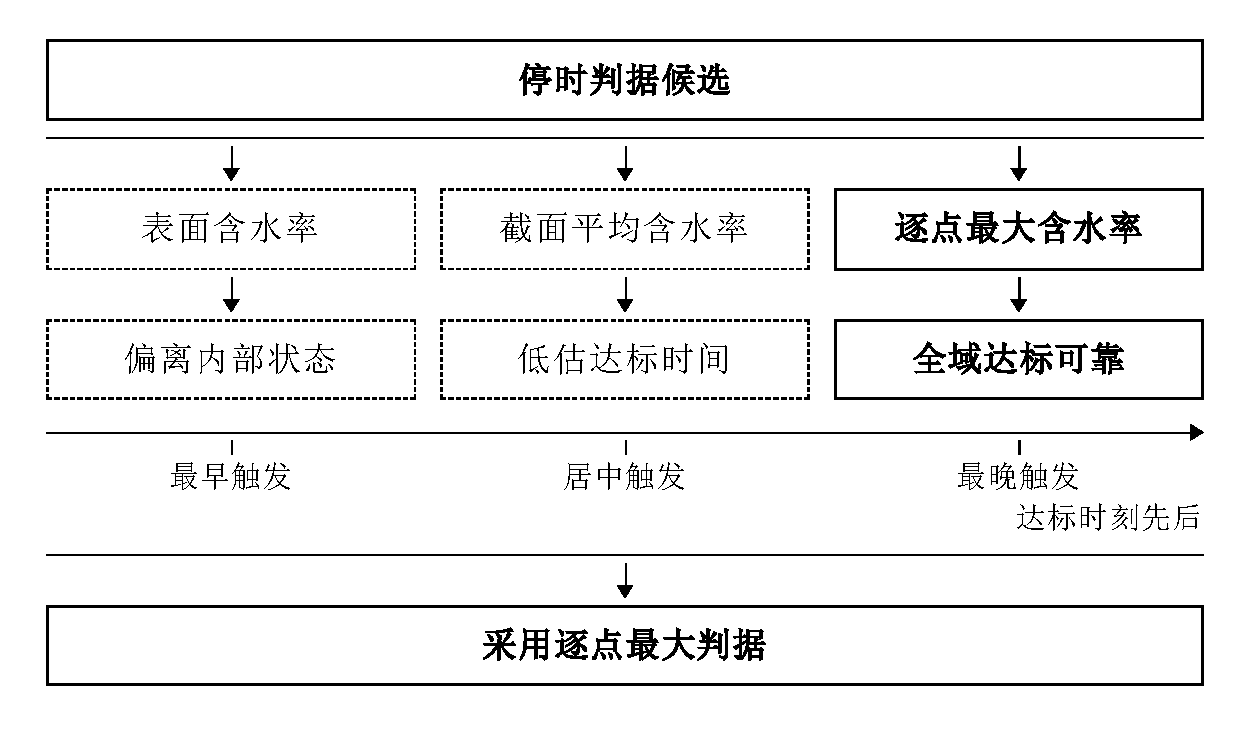
\includegraphics[width=0.9\textwidth,height=0.8\textheight,keepaspectratio]{../figures/fig_criterion_logic.pdf}
  \caption{停时判据的三候选决策。表面判据偏离内部状态，截面平均判据会低估达
  标时间，逐点最大判据能保证全域达标，故取后者；加粗框为采纳路径，虚线框为对照
  路径。底部时间轴只表示三种判据触发的先后次序，不含数值。}
  \label{fig:criterion-logic}
\end{figure}

图中底部时间轴上三个触发点的先后次序不依赖具体参数，它由三个判据量之间的不等关系直接决定。这一次序也说明误用前两种判据的后果是单向的：一定偏早，也就是把没有干透的药材判为合格。实算给出了这一偏差的量级，若改用截面平均含水率判据，达标时刻会提前 $21.70$~h，接近正确时长的四成。据此把烘干所需时间定义为

\begin{equation}
t_{\rm dry}=\inf\Big\{t>0:\ \max_{0\le r\le R_0}C(r,t)<C_{\rm th}\Big\},\qquad C_{\rm th}=0.15\ \mathrm{kg/kg}.
\label{eq:tdry}
\end{equation}

需要说明的是，判据写成径向最大值而不是中心值，是因为最湿位置的所在并非先验已知。本题在轴对称与外向失水的条件下，实算逐时刻核对确认 $\max_r C(r,t)$ 恒等于 $C(0,t)$，两者在 $10^{-12}$ 容差下完全一致，故最湿点始终在轴线；但判据的定义仍以最大值为准，这样在其他工况下也不会失效。

\subsection{停时的数值定位}

式~\eqref{eq:tdry} 是一个首次穿越时刻，它不能由某个显式表达式求出，只能在时间推进过程中逐步判断。求解流程如图~\ref{fig:flow-q3}。

\begin{figure}[htbp]
  \centering
  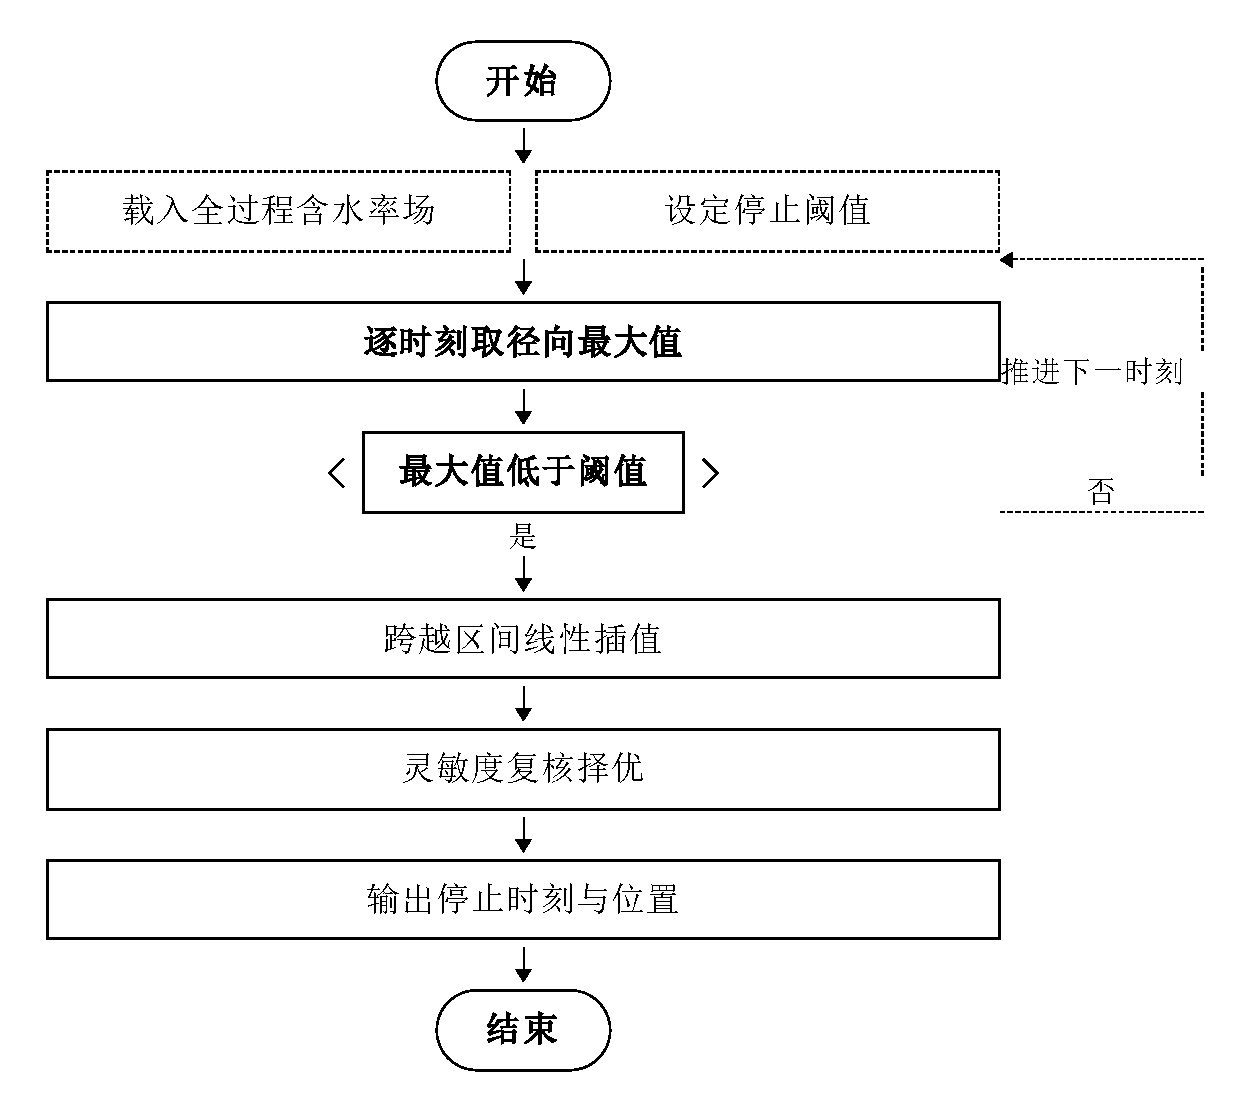
\includegraphics[width=0.86\textwidth,height=0.8\textheight,keepaspectratio]{../figures/fig_flow_q3.pdf}
  \caption{问题 3 停止时刻的判定流程。逐时刻取径向最大含水率与阈值比较，未达
  阈值则由右侧回路推进到下一时刻，已达阈值则在跨越区间内线性插值定位停时，再经
  灵敏度复核后输出。虚线框表示题给数据与外部给定的阈值。}
  \label{fig:flow-q3}
\end{figure}

流程的主体与问题二相同，新增的只是每步之后的一次比较和一次插值。由于输出间隔为 $60$~s，判据量恰好跨越阈值的那一刻一般落在两个输出时刻之间，需要在该区间内定位。设第 $k$ 个输出时刻的判据量仍高于阈值而第 $k+1$ 个已低于阈值，则按线性插值取

\begin{equation}
t_{\rm dry}=t_k+\frac{C_{\max}(t_k)-C_{\rm th}}{C_{\max}(t_k)-C_{\max}(t_{k+1})}\,\big(t_{k+1}-t_k\big).
\label{eq:interp}
\end{equation}

线性插值在此处足够可靠，因为判据量在阈值附近的下降速率极小且严格单调。实算的跨越区间为 $207060$ 至 $207120$~s，区间两端判据量分别为 $0.1500157$ 与 $0.1499982$，宽度恰为一个输出步，区间内不存在第二次穿越。

\subsection{烘干时长与全过程水分分布}

由式~\eqref{eq:interp} 定位得到

\begin{equation}
t_{\rm dry}=207113.776\ \mathrm{s}=57.5316\ \mathrm{h}=2.40\ \text{天}.
\label{eq:tdry3}
\end{equation}

该结果落在题目所述“烘干过程一般持续 2--3 天”的区间之内，为模型提供了一个来自题面本身的外部印证。达标时刻药材表面含水率已降至 $0.0526$~kg/kg，截面平均含水率为 $0.123903$~kg/kg，二者都远低于阈值，而轴线附近的含水率恰好抵达阈值。这一组数字正是“各处”与“平均”不能混用的直观说明：截面平均在轴线达标之前很久就已经跌破阈值。

按题目要求给出的水分浓度结果列于表~\ref{tab:q3C}。

\begin{table}[H]
\centering
\caption{药材烘干过程的水分浓度（单位：kg/kg）}\label{tab:q3C}
\begin{tabular}{cccccc}
\toprule
\multirow{2}{*}{时间/h} & \multicolumn{5}{c}{到药材中心的距离/cm}\\
\cmidrule(lr){2-6}
 & 0 & 0.5 & 1 & 1.5 & 2 \\
\midrule
6  & 1.0176 & 0.9888 & 0.9021 & 0.7555 & 0.5332 \\
12 & 0.4569 & 0.4439 & 0.4037 & 0.3303 & 0.1647 \\
18 & 0.2992 & 0.2919 & 0.2691 & 0.2256 & 0.0847 \\
24 & 0.2380 & 0.2330 & 0.2169 & 0.1857 & 0.0665 \\
30 & 0.2060 & 0.2020 & 0.1893 & 0.1642 & 0.0598 \\
36 & 0.1860 & 0.1826 & 0.1719 & 0.1505 & 0.0566 \\
42 & 0.1722 & 0.1692 & 0.1598 & 0.1408 & 0.0548 \\
48 & 0.1619 & 0.1593 & 0.1508 & 0.1335 & 0.0537 \\
54 & 0.1539 & 0.1515 & 0.1437 & 0.1278 & 0.0530 \\
烘干结束时间 & 0.1500 & 0.1477 & 0.1402 & 0.1249 & 0.0526 \\
\bottomrule
\end{tabular}

\vspace{0.6em}
\begin{minipage}{0.92\textwidth}
\footnotesize 末行为式~\eqref{eq:tdry3} 给出的烘干结束时间 $t_{\rm dry}=57.5316$~h。按式~\eqref{eq:tdry}
的定义，$t_{\rm dry}$ 正是判据量抵达阈值的时刻，故该行轴线处的数值等于阈值 $0.1500$；
严格低于阈值在其后的任意时刻成立，例如下一个输出时刻（晚 $6.2$~s）轴线含水率为
$0.1499982$~kg/kg。
\end{minipage}
\end{table}

% 同上：行内数学密集的中文段落，补一点应急伸展量。
{\emergencystretch=2.5em
表中数据呈现出显著的前快后慢：前 $12$~h 轴线含水率由 $2.5500$ 一路降到 $0.4569$~kg/kg，去掉了总降幅的八成以上；而从 $0.4569$ 降到阈值却用掉了剩下的 $45$~h。造成这一转折的正是扩散系数随变干而急剧减小。同时可以看到，表面在 $12$~h 时已降到 $0.1647$、$18$~h 时降到 $0.0847$~kg/kg，此后基本不再变化，而轴线仍在缓慢下降，整个后半程的进展几乎全部发生在药材内部。图~\ref{fig:q3-criterion} 给出三个判据量的完整下降过程与停时邻域的放大。\par}

\begin{figure}[htbp]
  \centering
  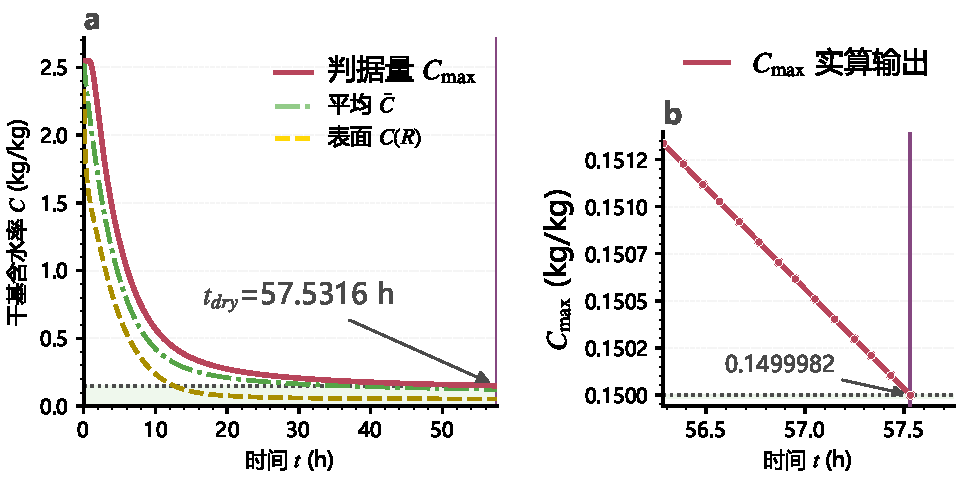
\includegraphics[width=0.9\textwidth,height=0.8\textheight,keepaspectratio]{../figures/fig_q3_criterion.pdf}
  \caption{问题 3 停时判据的实算依据。a：判据量 $\max_r C$、表面含水率与截面
  平均含水率三条曲线的全程下降，水平点线为阈值 0.15，绿色底带为达标区；三条
  曲线的先后次序印证了平均判据偏早、表面判据更偏早。b：停时前 1.25\,h 的邻域
  放大（1\,min 分辨率的实算输出点），显示判据被单调穿越且只穿越一次，故插值
  定位的停时唯一。轴对称条件下最湿位置恒在轴线，$\max_r C$ 即中心值。}
  \label{fig:q3-criterion}
\end{figure}

左图中三条曲线自上而下依次是判据量、截面平均和表面含水率，它们与阈值线的交点从右到左排列，与图~\ref{fig:criterion-logic} 所给的次序一致，且交点之间的水平距离相当可观，说明判据取法的影响不是可以忽略的细节。右图把停时前 $1.25$~h 放大后可以看到，实算输出点排成一条平缓且严格单调的直线，穿越阈值时既无震荡也无二次穿越，式~\eqref{eq:interp} 的线性插值在这样的局部形态下几乎没有额外误差。

最后把一维径向解按轴对称铺回圆截面，得到四个时刻的水分分布快照，见图~\ref{fig:q3-frames}。

\begin{figure}[htbp]
  \centering
  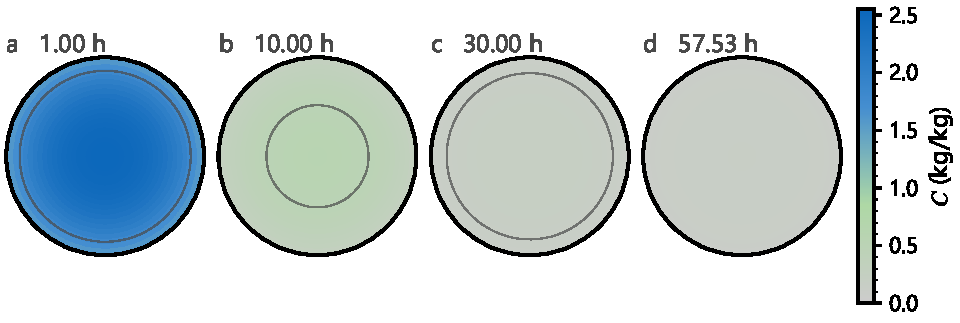
\includegraphics[width=0.9\textwidth,height=0.8\textheight,keepaspectratio]{../figures/fig_q3_frames.pdf}
  \caption{问题 3 圆截面水分场的四帧俯视快照（1、10、30\,h 与停时），把一维
  径向解按轴对称铺成圆盘。四帧共用同一色标以便跨帧比较，细等值线为 0.15、
  0.5、1.0、1.8 四级。干燥前沿由外向内推进，末帧整盘进入达标色域，直观说明
  全域达标是在最湿的轴线越过阈值那一刻实现的。}
  \label{fig:q3-frames}
\end{figure}

四帧连起来看，$1$~h 时只有薄薄一圈外缘变干，$10$~h 时干燥前沿已推进到半径中段，$30$~h 时整盘颜色接近均匀但轴心仍有一小块未达标，到停时那一帧才整盘进入达标色域。最后一帧中轴心残留的浅色斑点面积很小，却决定了整炉药材的出炉时刻，这正是逐点判据在工程上的意义所在。本问的截面水分总量平衡残差为 $5.5\times10^{-13}$，全程共 $3452$ 个输出时刻、每时刻 $21$ 个径向位置的完整水分场随结果文件一并给出。
